\documentclass[11pt]{article}

\usepackage[margin=1in]{geometry}
\usepackage{amsmath}
\usepackage{amssymb}
\usepackage{booktabs}
\usepackage{caption}
\usepackage{subcaption}
\usepackage{float}
\usepackage{xcolor}
\usepackage{listings}
\usepackage{pgfplots}
\usepackage{hyperref}
\pgfplotsset{compat=1.18}

\lstset{
  basicstyle=\ttfamily\small,
  frame=single,
  columns=fullflexible,
  keepspaces=true,
  xleftmargin=1em,
  xrightmargin=1em
}

\title{Milestone 3: Split-KV FlashAttention and\\Workload-Adaptive Kernel Selection on NVIDIA Ada GPUs}
% TODO: add all team members.
\author{Shaunak Aghor \and Sudeep Kalvakuntla}
\date{\today}

\begin{document}
\maketitle

\begin{abstract}
In Milestone 2 we implemented scaled dot-product attention in CUDA with three
separate kernels that store the full $M \times N$ score matrix in GPU memory.
In this milestone we implement a fused FlashAttention-style kernel that uses
tiling and online softmax, so the score matrix is never stored. We then
study two possible optimizations. First, we choose the tile size per input
shape with a lookup table built by offline tuning. This gives at most about
4\%, because every tile size has the same bottleneck. Second, we add
\emph{split-KV} (the idea behind FlashDecoding), which splits the keys of each
query row across several thread blocks and merges the partial results.
We found that plain FlashAttention is actually \emph{slower} than the naive kernels
for decoding-like inputs (one or a few queries attending to a long history),
because it leaves most of the GPU idle. Split-KV fixes this: on 29 held-out
test shapes, split-KV with our selector is on average \textbf{2.5$\times$} faster
than the naive kernels on an RTX 4060 Laptop GPU and \textbf{4.3$\times$} faster
on an RTX 5000 Ada, and up to 11.9$\times$ and 19.3$\times$ faster than plain
FlashAttention. Because the best number of splits depends on both the input
shape and the GPU, the selector now chooses between real alternatives, although
most of the gain comes from split-KV itself.
All variants are checked against a double-precision CPU reference
(322 test cases).
\end{abstract}

% ===========================================================================
\section{Introduction}

Attention is the core operation of transformer models. For queries
$Q \in \mathbb{R}^{M \times D}$, keys $K \in \mathbb{R}^{N \times D}$ and values
$V \in \mathbb{R}^{N \times D}$ it computes
\begin{equation}
  O = \mathrm{softmax}\!\left(\frac{QK^\top}{\sqrt{D}}\right) V .
\end{equation}
The straightforward GPU implementation (our Milestone 2) writes the score
matrix $S = QK^\top/\sqrt{D}$ to global memory, normalizes it with a second
kernel, and multiplies by $V$ in a third. The extra memory traffic and the
$O(MN)$ buffer make this slow and memory hungry for long sequences.

FlashAttention~\cite{dao2022flashattention,dao2023flashattention2} avoids this
by processing $K$ and $V$ in tiles that fit in on-chip shared memory and
computing the softmax \emph{online}, so $S$ is never stored.

Our target application is a chatbot. When a chatbot generates text, each new
step has only a few new query tokens ($M$ small, often $M=1$) but must attend
to the whole conversation history held in the KV cache ($N$ large). We found
that basic FlashAttention uses the GPU poorly in exactly this case.
This report describes:
\begin{enumerate}
  \item a fused FP32 FlashAttention kernel with causal masking, batches and heads;
  \item an offline-tuned selector that picks a kernel configuration per shape;
  \item split-KV, which fixes the poor GPU utilization for small $M$;
  \item measurements on two GPUs, including results that did \emph{not} work.
\end{enumerate}

% ===========================================================================
\section{Background}

\subsection{Online softmax}
Softmax over a row of scores $s_1,\dots,s_N$ needs the maximum $m=\max_j s_j$
(for numerical stability) and the sum $\ell = \sum_j e^{s_j - m}$.
Online softmax computes these in one pass over tiles of the row.
For each row we keep a running maximum $m$, a running sum $\ell$, and an
unnormalized output $o = \sum_j e^{s_j - m} v_j$. When a new tile with
scores $s_j$ arrives:
\begin{align}
  m' &= \max\!\left(m,\ \max_{j \in \text{tile}} s_j\right), \qquad
  c = e^{m - m'}, \\
  \ell' &= c\,\ell + \sum_{j \in \text{tile}} e^{s_j - m'}, \qquad
  o' = c\,o + \sum_{j \in \text{tile}} e^{s_j - m'}\, v_j .
\end{align}
The correction factor $c$ rescales everything computed so far to the new
maximum. After the last tile, $O = o/\ell$. The result is exact, not an
approximation.

\subsection{Causal masking for chunked prefill}
When $M$ new tokens are processed against $N$ keys (old history plus the new
chunk), query $i$ may attend to key $j$ only if $j \le N - M + i$
(``bottom-right'' alignment). For $M = N$ this is the usual causal mask, and
for $M = 1$ the single query sees every key.

% ===========================================================================
\section{Implementation}

The CUDA program is \texttt{src/attention.cu} and the experiment driver is
\texttt{scripts/experiment.py}, both in the \texttt{milestone3} folder.
Everything uses FP32 to match Milestone 2. Inputs are $Q$ of shape $[B, H, M, D]$ and $K, V$ of
shape $[B, H, N, D]$, with $D \in \{32, 64, 128\}$.

\subsection{Naive baseline (Milestone 2)}
We kept the Milestone 2 design (three kernels, $16 \times 16$ thread blocks,
one thread per softmax row) and extended it to batches, multiple heads,
rectangular shapes and causal masking. It needs a scratch buffer of
$B \cdot H \cdot M \cdot N$ floats.

\subsection{Fused FlashAttention kernel}
\begin{itemize}
  \item \textbf{One warp per query row.} Each of the 32 threads holds
        $D/32$ elements of the query and of the output row in registers.
  \item \textbf{One block = $R$ warps = $R$ query rows} ($R \in \{4, 8\}$).
        The block loads $T$ keys and values at a time
        ($T \in \{16, 32, 64\}$) into shared memory, and all $R$ warps reuse them.
  \item For each key in the tile the warp computes the dot product with a
        warp-shuffle reduction, then applies the online-softmax update.
  \item Blocks skip tiles that lie completely beyond their last allowed causal key.
\end{itemize}
We call a configuration ``$R{\times}T$'', e.g.\ \texttt{8x16}. The six
combinations are compiled as C++ template instances.

\subsection{Split-KV}
With the kernel above, the grid has only $\lceil M/R \rceil \cdot B \cdot H$
blocks and each block loops over all $N$ keys. For $M = 1$, $B = 1$, $H = 4$ that
is just 4 blocks, while the RTX 4060 Laptop GPU has 24 streaming
multiprocessors (SMs) and the RTX 5000 Ada has 100. Most of the GPU is idle,
and the run time is the time one block needs to walk through all $N$ keys.

Split-KV adds a third grid dimension of size $S$. Block $z$ processes only the
keys in $[zC, (z+1)C)$, where $C$ is a multiple of $T$. Each block writes its
unnormalized output $o_z$ and its statistics $(m_z, \ell_z)$ to a scratch
buffer. A second small kernel merges the $S$ partial results with the same
rescaling rule as online softmax:
\begin{equation}
  m = \max_z m_z, \qquad
  \ell = \sum_z \ell_z\, e^{m_z - m}, \qquad
  O = \frac{1}{\ell}\sum_z o_z\, e^{m_z - m}.
\end{equation}
Split 0 always contains key 0, which every row is allowed to see, so $m$ is
finite. A split that is completely masked reports $m_z = -\infty$, which gives
it weight $0$. The scratch buffer has $S \cdot B \cdot H \cdot M \cdot (D+2)$
floats, much smaller than the naive $M \times N$ score matrix.
A configuration with splits is written e.g.\ \texttt{8x16s4}; we allow
$S \in \{1, 2, 4, 8, 16, 32\}$.

\subsection{Selector}
The selector rounds $M$ and $N$ up to powers of two and looks up
$(B, H, M_\text{bucket}, N_\text{bucket}, D, \text{causal})$ in a table. If the
bucket is missing, it uses the best fixed configuration. The table is built
offline by \texttt{experiment.py tune}:
\begin{enumerate}
  \item Time every configuration on every training shape (3 rounds in random order).
  \item For each shape, divide each configuration's median time by the best one.
  \item The \emph{fixed} configuration minimizes the geometric mean of these
        ratios over all training shapes.
  \item For each bucket choose the best configuration, but keep the fixed one
        unless the other is at least 3\% faster (a simple guard against noise).
\end{enumerate}

% ===========================================================================
\section{Experimental Setup}

\begin{table}[H]
\centering
\caption{Hardware and software.}
\label{tab:hw}
\begin{tabular}{lll}
\toprule
 & RTX 4060 Laptop GPU & RTX 5000 Ada Generation \\
\midrule
Architecture / compute capability & Ada, 8.9 & Ada, 8.9 \\
SMs & 24 & 100 \\
Memory & 8 GB & 32 GB \\
System & Laptop, WSL2 & Lab workstation, Ubuntu 24.04 \\
CUDA (nvcc) & 12.0 & 12.0 \\
\bottomrule
\end{tabular}
\end{table}

\paragraph{Workloads.} The training set has 29 shapes and the held-out test set
has 29 different shapes (\texttt{workloads/train.csv} and \texttt{test.csv}).
They mimic chatbot prefill chunks ($M = 24\ldots512$) and decoding
($M = 1\ldots16$) with $N$ from 96 to 4096 keys, $H = 4$ heads, mostly causal.
Test shapes never equal training shapes. Most fall into a trained bucket,
and one (\,$B = 2$, $N = 3072$) checks the fallback.

\paragraph{Timing.} Each measurement is a separate process: warm-up runs, then
timed runs measured with CUDA events around the kernel launch(es). We report
the median. Every experiment repeats in 3 rounds in random order, and we take
the median over rounds. Host-to-device copies and memory allocation are not timed.

\paragraph{Correctness.} \texttt{experiment.py check} runs 7 small shapes
(sizes that are not multiples of the tile, one query, $M > N$, several heads) with
three input scales (all-equal scores, normal, very large scores) for every
configuration, plus the selector. Each output is compared with a
double-precision CPU implementation with tolerance
$|{\rm err}| \le 2\cdot10^{-4} + 2\cdot10^{-4}|{\rm ref}|$.

% ===========================================================================
\section{Results}

\subsection{Correctness}
All 322 cases pass on both GPUs. The largest absolute error was
$7.5 \times 10^{-6}$ on the RTX 4060 Laptop GPU.

\subsection{Lesson 1: timing on a laptop GPU is noisy}
Our first tuning run used 10 warm-up and 50 timed iterations. For 19 of
the 22 test shapes, the ``dynamic'' and ``fixed'' variants ran the
\emph{same} kernel, but the reported speedups still ranged from
$0.72\times$ to $1.40\times$. The repeated measurements formed two groups
about $1.4\times$ apart (e.g.\ 1961\,\textmu s vs.\ 2748\,\textmu s), which matches
the laptop GPU switching between clock levels. With 500--1000 warm-up
iterations, repeated runs of the same kernel agreed within a few percent.
All results below use the longer warm-up.

\subsection{Lesson 2: choosing the tile size barely matters}
Table~\ref{tab:tiles} shows all six tile configurations on the RTX 5000 Ada.
\texttt{8x16} is fastest or within 1\% on 22 of the 26 shapes we tried. The
exception is $D = 128$ with a small grid ($B \cdot H = 4$), where
\texttt{8x32} is about 3--4\% faster (the RTX 4060 shows the same preference).
With a large grid ($B \cdot H = 32$) this reverses and \texttt{8x16} is 20\%
faster, because an \texttt{8x32} block at $D = 128$ needs about 33\,KB of shared
memory, which limits how many blocks run on each SM.

\begin{table}[H]
\centering
\caption{GPU time (\textmu s) of the six tile configurations without split-KV
on the RTX 5000 Ada (selected shapes; causal; 1000 warm-up, 200 timed runs).}
\label{tab:tiles}
\begin{tabular}{lrrrrrr}
\toprule
Shape $(B,H,M,N,D)$ & 4x16 & 4x32 & 4x64 & 8x16 & 8x32 & 8x64 \\
\midrule
1,4,32,512,64     & 181  & 183  & 184  & \textbf{150}  & 151  & 153 \\
1,4,128,2048,64   & 1008 & 748  & 755  & \textbf{590}  & 595  & 607 \\
4,4,128,2048,64   & 960  & 1515 & 2212 & \textbf{806}  & 811  & 1286 \\
1,4,1,2048,64     & 696  & 707  & 713  & \textbf{547}  & 562  & 565 \\
16,8,32,512,64    & 466  & 591  & 1092 & \textbf{391}  & 400  & 498 \\
1,4,128,2048,128  & 1140 & 1112 & 2033 & 831  & \textbf{802}  & 817 \\
1,4,32,512,128    & 278  & 271  & 273  & 210  & \textbf{204}  & 205 \\
1,32,512,512,128  & 1540 & 3088 & 6108 & \textbf{1122} & 1342 & 2408 \\
\bottomrule
\end{tabular}
\end{table}

The reason is that every configuration has the same bottleneck: each block
streams \emph{all} keys through shared memory, and the cost per key does not
depend on $T$. Eight warps beat four everywhere (even for $M = 1$, where seven
of the eight warps have no query row) because more threads load each tile.
Since no tile size wins on some shapes and loses on others, a tile-size
selector has almost nothing to choose. We also noticed that on the RTX 5000 Ada,
$M = 32$, $64$ and $128$ all take the same time (Table~\ref{tab:tiles} and
the sweep below): the GPU is mostly idle. This led us to split-KV.

\subsection{Split-KV}
Figure~\ref{fig:splits} shows the GPU time as a function of the number of
splits $S$ for \texttt{8x16} tiles.

\begin{figure}[H]
\centering
\begin{subfigure}{0.49\textwidth}
\centering
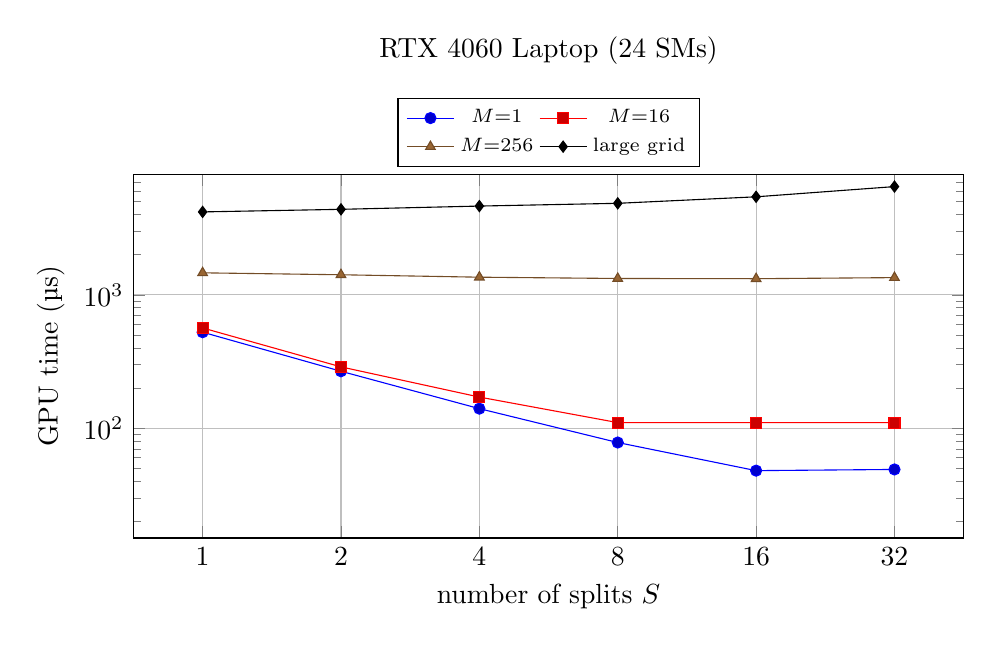
\begin{tikzpicture}
\begin{semilogyaxis}[
  width=\linewidth, height=6.2cm,
  xmode=log, log basis x=2,
  xtick={1,2,4,8,16,32}, xticklabels={1,2,4,8,16,32},
  xlabel={number of splits $S$}, ylabel={GPU time (\textmu s)},
  ymin=15, ymax=8000,
  legend style={font=\scriptsize, at={(0.5,1.02)}, anchor=south, legend columns=2},
  grid=major, title={RTX 4060 Laptop (24 SMs)}, title style={yshift=7ex}]
\addplot+[mark=*] coordinates {(1,524) (2,267) (4,140) (8,78) (16,48) (32,49)};
\addplot+[mark=square*] coordinates {(1,564) (2,288) (4,171) (8,110) (16,110) (32,110)};
\addplot+[mark=triangle*] coordinates {(1,1461) (2,1413) (4,1355) (8,1325) (16,1320) (32,1345)};
\addplot+[mark=diamond*] coordinates {(1,4183) (2,4374) (4,4627) (8,4852) (16,5429) (32,6476)};
\legend{$M{=}1$, $M{=}16$, $M{=}256$, large grid}
\end{semilogyaxis}
\end{tikzpicture}
\end{subfigure}
\hfill
\begin{subfigure}{0.49\textwidth}
\centering
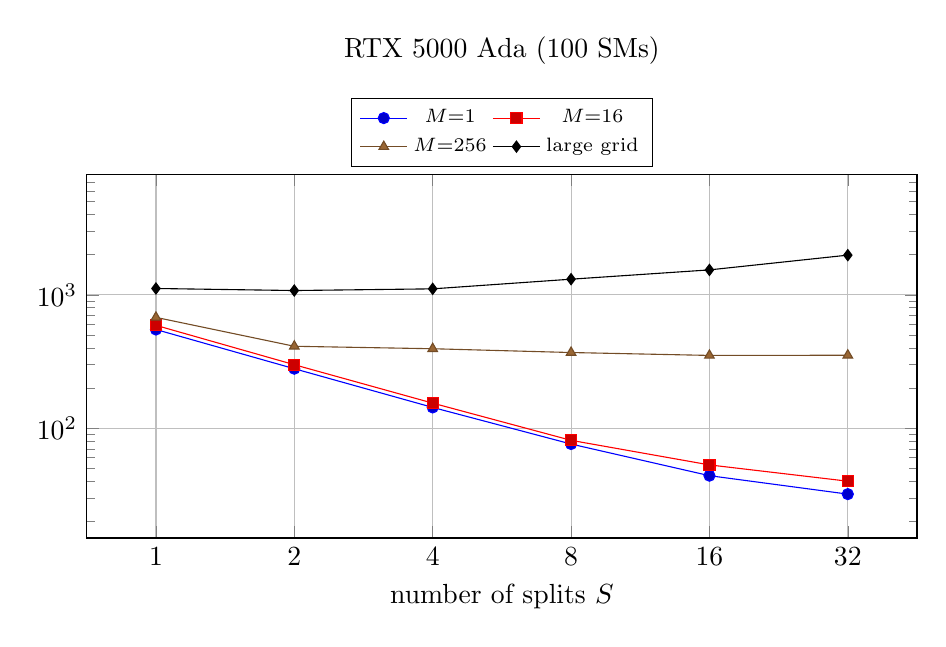
\begin{tikzpicture}
\begin{semilogyaxis}[
  width=\linewidth, height=6.2cm,
  xmode=log, log basis x=2,
  xtick={1,2,4,8,16,32}, xticklabels={1,2,4,8,16,32},
  xlabel={number of splits $S$},
  ymin=15, ymax=8000,
  legend style={font=\scriptsize, at={(0.5,1.02)}, anchor=south, legend columns=2},
  grid=major, title={RTX 5000 Ada (100 SMs)}, title style={yshift=7ex}]
\addplot+[mark=*] coordinates {(1,549) (2,279) (4,143) (8,76) (16,44) (32,32)};
\addplot+[mark=square*] coordinates {(1,590) (2,299) (4,154) (8,81) (16,53) (32,40)};
\addplot+[mark=triangle*] coordinates {(1,677) (2,411) (4,394) (8,369) (16,351) (32,352)};
\addplot+[mark=diamond*] coordinates {(1,1115) (2,1076) (4,1108) (8,1309) (16,1537) (32,1983)};
\legend{$M{=}1$, $M{=}16$, $M{=}256$, large grid}
\end{semilogyaxis}
\end{tikzpicture}
\end{subfigure}
\caption{GPU time vs.\ number of key splits (log scales, \texttt{8x16} tiles,
causal). $M{=}1$, $16$, $256$ use $B{=}1$, $H{=}4$, $N{=}2048$, $D{=}64$.
``Large grid'' is $B{=}1$, $H{=}32$, $M{=}N{=}512$, $D{=}128$.
1000 warm-up and 200 timed runs per point.}
\label{fig:splits}
\end{figure}

\begin{itemize}
  \item \textbf{Decoding becomes much faster.} For $M = 1$, $N = 2048$ the time
        drops from 524 to 48\,\textmu s on the RTX 4060 ($10.9\times$) and from 549 to
        32\,\textmu s on the RTX 5000 Ada ($17\times$). Without split-KV our fused kernel
        was even slower than the naive Milestone 2 kernels for $M = 1$,
        because those kernels use many threads across the keys.
  \item \textbf{The best $S$ depends on the shape.} Small $M$ wants many splits.
        With a large grid the GPU is already full, and splitting only adds the
        merge step and extra memory traffic (up to $1.5\times$ slower on the 4060).
  \item \textbf{The best $S$ depends on the GPU.} For $M = 16$, the RTX 4060
        stops improving at $S = 8$ (110\,\textmu s), while the RTX 5000 Ada, with about
        $4\times$ more SMs, keeps improving up to $S = 32$ (40\,\textmu s).
\end{itemize}

\subsection{Tuning: how far is each configuration from the best?}
Table~\ref{tab:tuning} shows the tuning objective: for each configuration,
the geometric mean (over the 29 training shapes) of its time divided by the
fastest configuration for that shape. A value of 1.00 would mean ``always the
fastest''. Without split-KV, even the best tile is on average $2.3\times$
(RTX 4060) and $4.6\times$ (RTX 5000 Ada) slower than the best choice; the
larger GPU suffers more because more of it is idle. \texttt{8x32} and
\texttt{8x16} are within 3--6\% of each other, which agrees with
Table~\ref{tab:tiles}.

\begin{table}[H]
\centering
\caption{Tuning objective (lower is better; 1.00 = fastest on every shape).
Each value is a geometric mean over 29 training shapes, 3 rounds, 500 warm-up and 100 timed runs.}
\label{tab:tuning}
\begin{tabular}{lrr}
\toprule
Configuration & RTX 4060 Laptop & RTX 5000 Ada \\
\midrule
\texttt{8x16s32} & 1.12 & \textbf{1.09} \\
\texttt{8x16s16} & \textbf{1.06} & \textbf{1.09} \\
\texttt{8x32s8}  & 1.10 & 1.28 \\
\texttt{8x16s8}  & 1.13 & 1.31 \\
\texttt{8x16s4}  & 1.29 & 1.75 \\
\texttt{8x16s2}  & 1.70 & 2.81 \\
\midrule
\texttt{8x32} (best without split-KV) & 2.26 & 4.61 \\
\texttt{8x16} & 2.32 & 4.88 \\
\texttt{4x16} & 2.72 & 5.57 \\
\texttt{4x64} & 4.08 & 6.13 \\
\bottomrule
\end{tabular}
\end{table}

The tuner picked \texttt{8x16s16} as the best fixed configuration on the RTX 4060
and \texttt{8x16s32} on the RTX 5000 Ada: the larger GPU needs more blocks to be
filled. The selector tables use five different configurations on each GPU
(4 to 32 splits, \texttt{8x16} or \texttt{8x32} tiles), unlike the tile-only
experiment where almost every bucket chose the same tile.

\subsection{End-to-end benchmark on held-out shapes}
\label{sec:bench}
We compare four variants on the 29 held-out test shapes:
\textbf{naive} (Milestone 2 kernels),
\textbf{flash} (plain FlashAttention, best configuration without splits: \texttt{8x32}),
\textbf{fixed} (best single configuration, with split-KV), and
\textbf{dynamic} (configuration chosen per shape by the selector).
Table~\ref{tab:bench-summary} summarizes the speedups and
Table~\ref{tab:bench-shapes} shows selected shapes.

\begin{table}[H]
\centering
\caption{Geometric-mean GPU speedups on the 29 held-out test shapes
(3 rounds, 500 warm-up, 100 timed runs). ``A vs B'' $>1$ means A is faster.}
\label{tab:bench-summary}
\begin{tabular}{lrrr@{\hskip 2em}rrr}
\toprule
 & \multicolumn{3}{c}{RTX 4060 Laptop} & \multicolumn{3}{c}{RTX 5000 Ada} \\
 & all & $M \le 16$ & $M > 16$ & all & $M \le 16$ & $M > 16$ \\
\midrule
flash vs naive   & 1.13 & 0.43 & 1.64 & 0.97 & 0.39 & 1.36 \\
dynamic vs flash & 2.19 & 6.38 & 1.45 & 4.49 & 11.04 & 3.18 \\
dynamic vs naive & \textbf{2.48} & 2.76 & 2.38 & \textbf{4.33} & 4.30 & 4.34 \\
dynamic vs fixed & 1.04 & 1.02 & 1.04 & 1.06 & 1.03 & 1.07 \\
\bottomrule
\end{tabular}
\end{table}

\begin{table}[H]
\centering
\caption{GPU time (\textmu s) for selected held-out shapes ($H=4$, causal).
The configuration chosen by the selector is shown in brackets.}
\label{tab:bench-shapes}
\small
\begin{tabular}{lrrrl@{\hskip 1.5em}rrrl}
\toprule
 & \multicolumn{4}{c}{RTX 4060 Laptop} & \multicolumn{4}{c}{RTX 5000 Ada} \\
Shape $(B,M,N,D)$ & naive & flash & dynamic & & naive & flash & dynamic & \\
\midrule
1, 1, 1536, 64   & 143  & 363  & 36   & [\texttt{8x16s16}] & 137  & 376  & 28  & [\texttt{8x16s32}] \\
1, 1, 3500, 64   & 310  & 824  & 70   & [\texttt{8x16s16}] & 306  & 853  & 44  & [\texttt{8x16s32}] \\
1, 12, 1536, 64  & 221  & 388  & 75   & [\texttt{8x32s8}]  & 194  & 400  & 34  & [\texttt{8x16s32}] \\
1, 24, 1536, 128 & 531  & 495  & 143  & [\texttt{8x16s16}] & 396  & 513  & 51  & [\texttt{8x16s32}] \\
1, 96, 1536, 64  & 935  & 441  & 378  & [\texttt{8x32s8}]  & 641  & 401  & 118 & [\texttt{8x16s32}] \\
1, 384, 384, 64  & 750  & 252  & 225  & [\texttt{8x32s4}]  & 438  & 116  & 70  & [\texttt{8x32s8}] \\
4, 96, 1536, 64  & 2251 & 1475 & 1434 & [\texttt{8x32s4}]  & 947  & 455  & 380 & [\texttt{8x32s8}] \\
2, 96, 3072, 64$^\ast$ & 2662 & 1720 & 1525 & [\texttt{8x16s16}] & 1447 & 799 & 392 & [\texttt{8x16s32}] \\
\bottomrule
\multicolumn{9}{l}{\footnotesize $^\ast$ Bucket not in the table, so the selector falls back to the fixed configuration.}
\end{tabular}
\end{table}

\paragraph{Observations.}
\begin{itemize}
  \item \textbf{Plain FlashAttention is not always faster than naive.} For
        $M \le 16$ it is about $2.5\times$ \emph{slower} on both GPUs, and on the
        RTX 5000 Ada it is slightly slower overall (0.97). The naive kernels launch
        one thread per (query, key) pair, so they use the whole GPU even for
        $M = 1$, while plain FlashAttention launches only a few blocks.
  \item \textbf{Split-KV fixes this.} With the selector, attention is on average
        $2.5\times$ (RTX 4060) and $4.3\times$ (RTX 5000 Ada) faster than naive, and
        it is faster than naive on \emph{every} test shape on both GPUs. Compared with
        plain FlashAttention the speedup is up to $11.9\times$ (RTX 4060) and
        $19.3\times$ (RTX 5000 Ada), for the single-query shapes.
  \item \textbf{Most of the benefit comes from split-KV itself.} The best single
        split configuration already captures most of the gain; choosing per shape
        adds a further 4\% (RTX 4060) and 6\% (RTX 5000 Ada) on average. Per shape
        it ranges from $0.85\times$ to $1.17\times$ on the RTX 4060 and from
        $0.91\times$ to $1.59\times$ on the RTX 5000 Ada, with 2 and 3 shapes
        respectively more than 3\% slower than the fixed configuration. Those
        losses come from buckets tuned on a single training shape.
  \item \textbf{The selector's choices depend on the GPU.} For the same test shape
        the RTX 5000 Ada usually picks more splits than the RTX 4060
        (Table~\ref{tab:bench-shapes}), as expected from its $4\times$ larger SM count.
\end{itemize}

% ===========================================================================
\section{Discussion and Limitations}

\begin{itemize}
  \item Our kernel is educational. It uses FP32 CUDA cores, no Tensor Cores, and
        no backward pass. One warp-shuffle reduction per key is its main cost.
        It is not meant to compete with the official FlashAttention-2.
  \item Split-KV and choosing the number of splits from the GPU size are known
        ideas (FlashDecoding; FlashAttention-2 picks the number of splits with a
        heuristic based on the SM count). Our contribution is implementing them on
        top of our own kernel and measuring when they help on two GPUs.
  \item The selector is a lookup table built from one or a few training shapes
        per bucket. More shapes per bucket would make its choices more robust.
  \item Each measurement runs in its own process with warmed-up buffers. We do
        not measure a real serving system (KV-cache updates, batching of
        requests, tokens per second).
  \item The laptop GPU's clock changes add noise; a long warm-up was necessary.
\end{itemize}

% ===========================================================================
\section{Conclusion}

A fused FlashAttention kernel removes the $O(MN)$ score buffer of our
Milestone 2 implementation and is faster for prefill-sized inputs, but it is
slower than the naive kernels when there are only a few queries. Choosing
the tile size per shape gave almost nothing (at most about 4\%), because all
tile sizes share the same bottleneck: one block walks through all keys.
Splitting the keys across blocks removes that bottleneck. On held-out shapes it
makes attention $2.5\times$ (RTX 4060 Laptop) and $4.3\times$ (RTX 5000 Ada) faster
than naive on average, and up to $19\times$ faster than plain FlashAttention for
single-query attention. The best number of splits depends on the shape and the
GPU; choosing it per shape with our selector adds a further 4--6\% over the best
fixed choice.

% TODO: if your course asks for it, add a note on the tools/assistance you used.

\begin{thebibliography}{9}
\bibitem{dao2022flashattention}
T.~Dao, D.~Y. Fu, S.~Ermon, A.~Rudra, and C.~R\'e,
``FlashAttention: Fast and memory-efficient exact attention with IO-awareness,''
\emph{NeurIPS}, 2022. \url{https://arxiv.org/abs/2205.14135}

\bibitem{dao2023flashattention2}
T.~Dao, ``FlashAttention-2: Faster attention with better parallelism and work
partitioning,'' 2023. \url{https://arxiv.org/abs/2307.08691}

\bibitem{flashdecoding}
T.~Dao, D.~Haziza, F.~Massa, and G.~Sizov, ``Flash-Decoding for long-context
inference,'' 2023. \url{https://crfm.stanford.edu/2023/10/12/flashdecoding.html}

\bibitem{triton}
Triton fused attention tutorial.
\url{https://triton-lang.org/main/getting-started/tutorials/06-fused-attention.html}

\bibitem{vllm}
vLLM documentation, chunked prefill.
\url{https://docs.vllm.ai/en/latest/configuration/optimization/}
\end{thebibliography}

\end{document}
